%!TEX root = main.tex
\chapter{Bundle Adjustment}\label{chapter:Bundle Adjustment}
Bundle Adjustment(BA) is a large, nonlinear least-squares problem that was presented by Triggs \cite{triggs2000bundle}. It is often solved as the last step of feature-based structure and motion (SfM) estimation in computer vision algorithms to refine the obtained estimation.\\
Structure from Motion (SfM) or 3D reconstruction can be defined as a problem of using 2D feature points that extract from  set of images depicting the same scene from different viewpoints. It tries to derive the 3D points of environment as well as the camera pose (extrinsic parameters) and the optical characteristics of the camera (camera matrix or intrinsic).
BA amounts to an optimization problem on the 3D structure and viewing parameters (i.e., camera pose and possibly intrinsic
calibration and radial distortion), to obtain a reconstruction which is optimal under certain assumptions regarding the noise pertaining to the observed image feature points. \\
The general idea behind the BA is to minimize the reprojection error between the observed and predicted image points, which is expressed as the sum of squares of a large number of nonlinear functions. Thus, the minimization is achieved using nonlinear least-squares algorithms. Levenberg-Marquardt (LM) is of the most successful due to its ease of implementation and its use of an effective damping strategy that lends it the ability to converge quickly from a wide range of initial guesses to the final goal.\\
In the case of time and memory, The general least-squares algorithm acquires high computational and memory storage costs Due to the very large number of parameters involved. But fortunately, the lack of interaction among certain subgroups of parameters results in the corresponding Jacobian being sparse, due to achieve considerable computational savings.\\
In this master thesis we do not want to go deep inside the math base of BA. There are so many libraries that already implemented the Bundle Adjustment. In this master thesis, the cvsba \footnote{\url{http://www.uco.es/investiga/grupos/ava/node/39}} (an OpenCV wrapper for sba library) ,which is an OpenCV wrapper for the well-known Sparse Bundle Adjustment library, was ported to Ubitrack Framework. This Bundle Abstemiousness is used to refine the 3D Points that estimated from mapping task of both marker-based and feature based techniques in Ubitrack.\\

\section{cvsba}
casbah is an open source library for Sparse Bundle Adjustment (sba) that based on OpenCV\footnote{\url{http://www.uco.es/investiga/grupos/ava/node/39}}. It was implemented by Manolis Lourakis at Foundation for Research and Technology - Hellas in Heraklion, Crete, Greece. The main features of this BA are:
\begin{itemize}
\item Based on sba-1.6, one of the most popular and robust bundle adjustment implementation, which is extensively used and tested by the community
\item sba installation is not needed since it is included in cvsba
\item New CMake structure which makes the library compilation, installation and linkage easier
\item Similar interface than Bundle Adjustment implementation on cv::LevMarqSparse::bundleAdjust()
\item Include examples to test the library on synthetically generated data
\item GPL license
\end{itemize}

\subsection{Usage}
The executive function of cvsba is \detokenize{Sba::run()}. 
\lstset{ %
	language=C++,                	% choose the language of the code
	basicstyle=\footnotesize,       % the size of the fonts that are used for the code
	keywordstyle=\color{black},  	% the color of keyword of language
	stringstyle=\color{black},		% the color of string line
	commentstyle=\color{black},		% the color of command line
	% numbers=left,                   % where to put the line-numbers
	numberstyle=\footnotesize,      % the size of the fonts that are used for the line-numbers
	stepnumber=1,                   % the step between two line-numbers. If it is 1 each line will be numbered
	% numbersep=5pt,                  % how far the line-numbers are from the code
	backgroundcolor=\color{white},  % choose the background color. You must add \usepackage{color}
	showspaces=false,               % show spaces adding particular underscores
	showstringspaces=false,         % underline spaces within strings
	showtabs=false,                 % show tabs within strings adding particular underscores
	% frame=single,           % adds a frame around the code
	tabsize=2,          % sets default tabsize to 2 spaces
	captionpos=b,           % sets the caption-position to bottom
	breaklines=true,        % sets automatic line breaking
	breakatwhitespace=false,    % sets if automatic breaks should only happen at whitespace
	escapeinside={\%*}{*)}          % if you want to add a comment within your code
}

\begin{lstlisting}
double Sba::run (  std::vector<cv::Point3d>& points,
                   const std::vector<std::vector<cv::Point2d> >& imagePoints,
                   const std::vector<std::vector<int> >& visibility,
                   std::vector<cv::Mat>& cameraMatrix,
                   std::vector<cv::Mat>& R,
                   std::vector<cv::Mat>& T,
                   std::vector<cv::Mat>& distCoeffs );

\end{lstlisting} \label{lst:cvsba}
For the M cameras and N 3D points, the parameters description is the following:
\begin{itemize}
\item \textbf{points:} The vector of estimated 3D points. Type:[input/outpu], Size:[N]
\item \textbf{imagePoints:} The observed 2D points of a same scene but with different viewpoints (cameras). It is notable that the size of 3D points and 2D points for each camera should be the same. As the other fact, they are the image projection of 3D points in each camera. Type:[input/outpu], Size:[M*N]
\item \textbf{visibility:} Is a vector of vector of int and the same size of imagePoints. Each element is 1 if points[j] is visible on camera i, otherwise it is 0. Type:[input], Size:[M*N] 
\item \textbf{cameraMatrix:} Is a vector of camera intrinsic matrix. Type:[input/output], Size:[M * (3*3)]
\item \textbf{R:} The rotation matrix of each camera. Type:[input/output], Size:[M * (3*3)]
\item \textbf{T:} the translation vector of each camera. Type:[input/output], Size:[M * (3*1)]
\item \textbf{distCoeffs:} It represents the distortion coefficients of each camera. Type:[input/output], Size:[M * (5*1)]
\item \textbf{return value:} The return value represents the reprojection error after the bundle adjustment.
\end{itemize}

\subsection{Type of optimization} \label{subsec:type_of_optimization}
The sba library can run different types of optimizations (\detokenize{Sba::MOTION}, \detokenize{Sba::STRUCTURE}, \detokenize{Sba::MOTIONSTRUCTURE}). Each type of optimization affect to some of the input parameters. For instance, MOTIONSTRUCTURE is aimed at modifying both the structure (3D points), and the motion (Intrinsics,Distortion , R and T). However, you can control which of these elements to be effectively optimized using fixedIntrinsics and fixedDistortion. If you set this parameters to 5, then Intrinsics and Distortion will not be modified at all. Then, the algorithm will only modify the 3D points. However, if you set  fixedIntrinsics and fixedDistortion to 0, then,  the the elements in cameraMatrix,R,T, distCoeffs will also be modified with the new optimized values.

\subsection{Parameters}
cvsba library and \detokenize{Sba::run()} can be executed by variety of parameters. \detokenize{Sba::Params} is a structure that consists of below parameters:
\begin{itemize}
\item \textbf{Type:} It represents the type of bundle adjustment that mentioned in previous subsection. This parameters is a Enum data structure with default value MOTIONSTRUCTURE for optimization.
		\begin{itemize}
			\item MOTIONSTRUCTURE: Both structure {3D points} and motion {R and T} are optimized. The value of that is 0.
			\item MOTION: The rotation and translation are optimized. The 3D points are fixed. The value in Enum is 1.
			\item STRUCTURE: The rotation and translation are kept fixed and 3D points optimized. Value of that is 2. 
		\end {itemize}
\item \textbf{iterations:} The number of iteration that is necessary for optimization. Default value is 150 iteration.
\item \textbf{minError:} The minimum reprojection error for termination the process.
\item \textbf{fixedIntrinsics:} Number of intrinsics parameters that are kept fixed [0-5] in the following order: [fx, cx, cy, fy/fx, s].
\item \textbf{fixedDistortion:} Number of distortion parameters that are kept fixed [0-5] in the following order: [k1, k2, p1, p2, k3].
\end{itemize}

\section{Our Implementation}
The cvsba was implemented based on OpenCV library. Therefor the data structure of all parameters are used of OpenCV. One part of this master's thesis is assigned to port the cvsba into Ubitrack Framework. Changing the data structure from OpenCV to Ubitrack and vice versa were one of the complicated part of this master thesis. The origin of Ubitarck is right-hand side whereas the openCV is left-hand side. Then all data should be converted from right-hand site to left-hand site and vice versa.The other difference between these two libraries is the origin of their coordinate systems. The position of origin (0,0) of image in Ubitrack is in lower left corner while the position of image origin is upper left corner. So all data relative to images such as feature points also should be converted to other coordinate system.\\
In the following the conversion functions that convert the data structures between the OpenCV and Ubitrack are described:
\begin{itemize}
\item \textbf{copyUbitrackVec2cvPoint3d:} converts the 3D points from  (\detokenize{std::vector < Ubitrack::Math::Vector < T, 3 > > &}) of Ubitrack to (\detokenize{std::vector <cv::Point3d> &}) of OpenCV. 
\item \textbf{copyUbitrackVec2cvPoint2d:} converts all observed 2D points from (\detokenize{std::vector < std::vector < Ubitrack::Math::Vector < T, 2 > > > &}) to (\detokenize{std::vector < std::vector <cv::Point2d> > &}).
\item \textbf{copyUbitrackMatrix2cvMat:} convert the Ubitrack (\detokenize{std::vector <Ubitrack::Math::Matrix <T, 3, 3> > &}) matrix to (\detokenize{std::vector <cv::Mat> &}). This function is used for converting the both intrinsic and rotation matrices.
\item \textbf{copyUbitrackVec2cvMat:} to convert the (\detokenize{std::vector <Ubitrack::Math::Vector< T, 3 > > &}) as the translation matrix to (\detokenize{std::vector <cv::Mat> &}) as a OpenCV matrix.
\item \textbf{makeVisibilityVec:} create a (\detokenize{std::vector <int>}) that consists of 1 and 0. These numbers represent that a relative projected point is visible in our image or no.
\item \textbf{copyCvPoint3d2UbitrackVec3:} To convert the optimized 3D points from the OpencCV system to Ubitrack Framework. It is not necessary to convert the rest matrices or vectors from OpenCV to Ubitrack because in all cases, the 3D points are optimized (The type of optimization is \detokenize{Sba::STRUCTURE}).
\end{itemize}

Except of converting the 2D points for matching the coordinate system between Ubitrack and OpenCV, the rotation and translation matrices also should be rotated $180 ^{\circ}$ around the Z axis. The conversion matrix for rotation is defined as below:
\begin{gather*}
	Rotation_{(Ubitrack)} = R_{z}(180) * Rotation_{(OpenCV)}\\
	and\\
    Rotation_{(OpenCV)} = R_{z}(180) * Rotation_{(Ubitrack)}
\end{gather*}
And for translation is:
\begin{gather*}
	Translation{(Ubitrack)} = R_{z}(180) * Translation{(OpenCV)}\\
	and\\
    Translation{(OpenCV)} = R_{z}(180) * Translation{(Ubitrack)}
\end{gather*}
Where 
\begin{gather*}
	R_{z}(180) = \begin{bmatrix}
       -1 & 0 & 0   \\[0.3em]
       0 & -1 & 0   \\[0.3em]
       0  & 0 & 1
     \end{bmatrix}
\end{gather*}

After converting the 2D points, rotation and translation matrices from Ubitrack to OpenCV, the \detokenize{Sba::run()} function is executed. Then the optimized 3D points converted again to Ubitrack and the process of Bundle Adjustment finishes.\\

\section{Result evaluation}
In this section the performance of cvsba and our porting module is evaluated. For this purpose, the estimated 3D points from Ubitrack marker-based pose estimation are optimized and compared by the ground true data. The Ubitrack marker-based pose estimation was implemented by Sven Barth as a master's thesis in Fachgebeit Augmented Reality (FAR) at technical university of Munich with title "A Flexible and Extensible Feature Tracking Architecture for the Ubitrack Framework". This feature tracking technique is inspired of PTAM \cite{klein2007parallel} and it works as follow: Firstly, The corners of markers detects reliably and accurately in each frame. Then marker id and their corners matched with previous frames. For instance the corners of marker "0272" in frame i matched with the corner of same marker in frame j. After that the correspondence 3D points of these corners are estimated by a 3D reconstruction approach and the pose of camera calculated.\\
To evaluate the performance of our module for using of cvsba bundle adjustment, after the second frames and when the 3D points of all marker's corners are estimated, the bundle adjustment module is executed to refine the estimated 3D points. The ground truth data is 3D points are provided by Farco machine in which its measurement error is 0.1 millimeters. The bundle adjustment procedure optimize the 3D points after second frames and our python evaluation script compare optimized 3D points wit ground truth data.\\
The data set is a video sequence that grabs from a board which consists of 10 markers with different id. \autoref{fig:marker_ground_truth} shows some example image of our test data set.
\begin{figure}[H]  
\begin{tabular}{cc}
  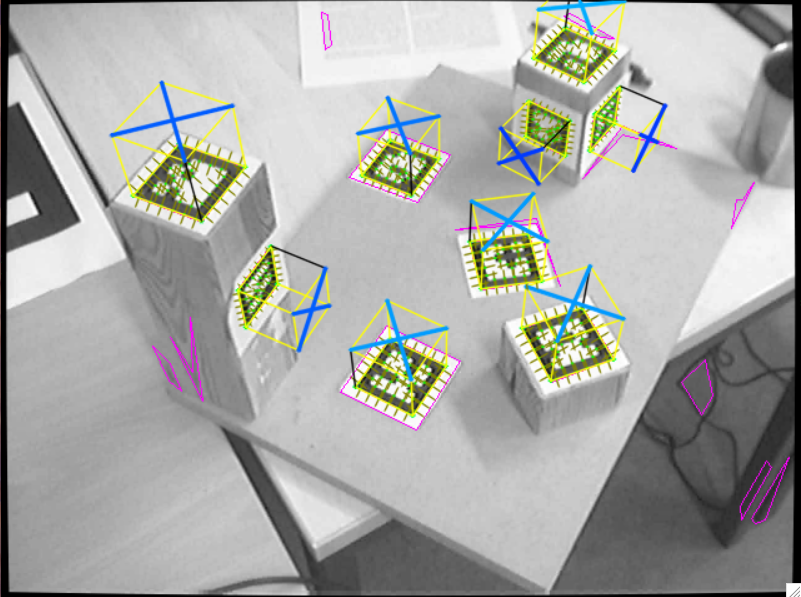
\includegraphics[width=65mm]{figures/marker_frame_1} &  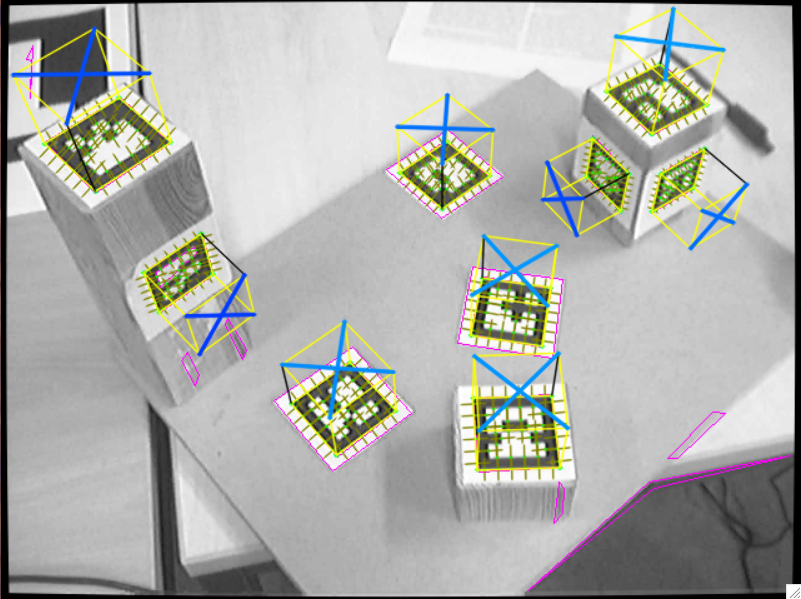
\includegraphics[width=65mm]{figures/marker_frame_2} \\
(a) sample 1 & (b) sample 2 \\[6pt]
  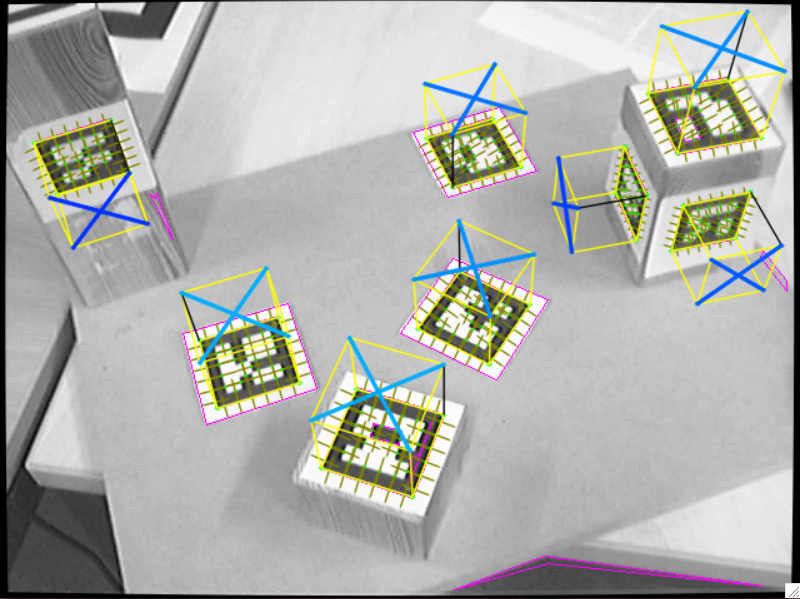
\includegraphics[width=65mm]{figures/marker_frame_3} &  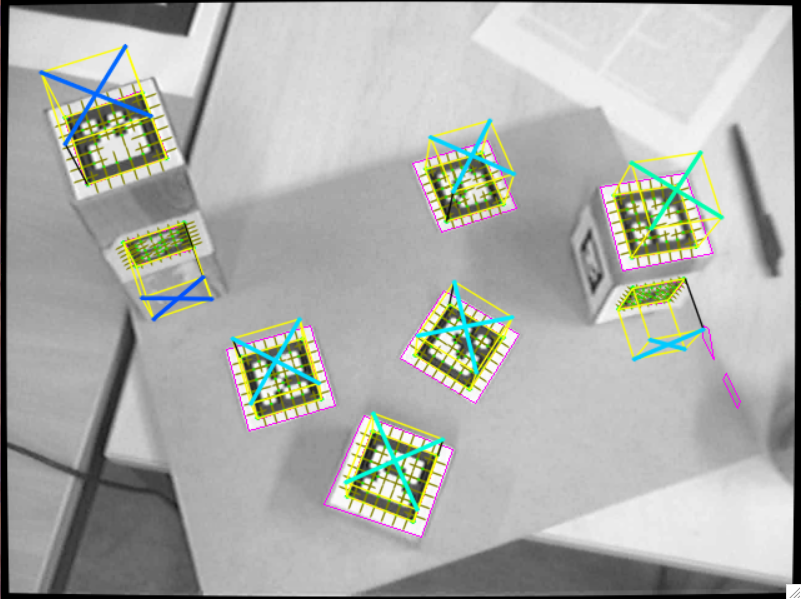
\includegraphics[width=65mm]{figures/marker_frame_4} \\
(c) sample 3 & (d) sample 4 \\[6pt]
\end{tabular}
\caption{Some sample of marker data set}\label{fig:marker_ground_truth}
\end{figure}

For evaluation, we create two sample data sets that each of them involves ten images. the images in each sample data set selected randomly from our data set. For each sample data set, the euclidean error of all four points of each markers are calculated compare to the ground truth. These euclidean errors draw on a graph after each step of optimization.

\subsection{Test 1}
\begin{figure}[H]
  \centering
  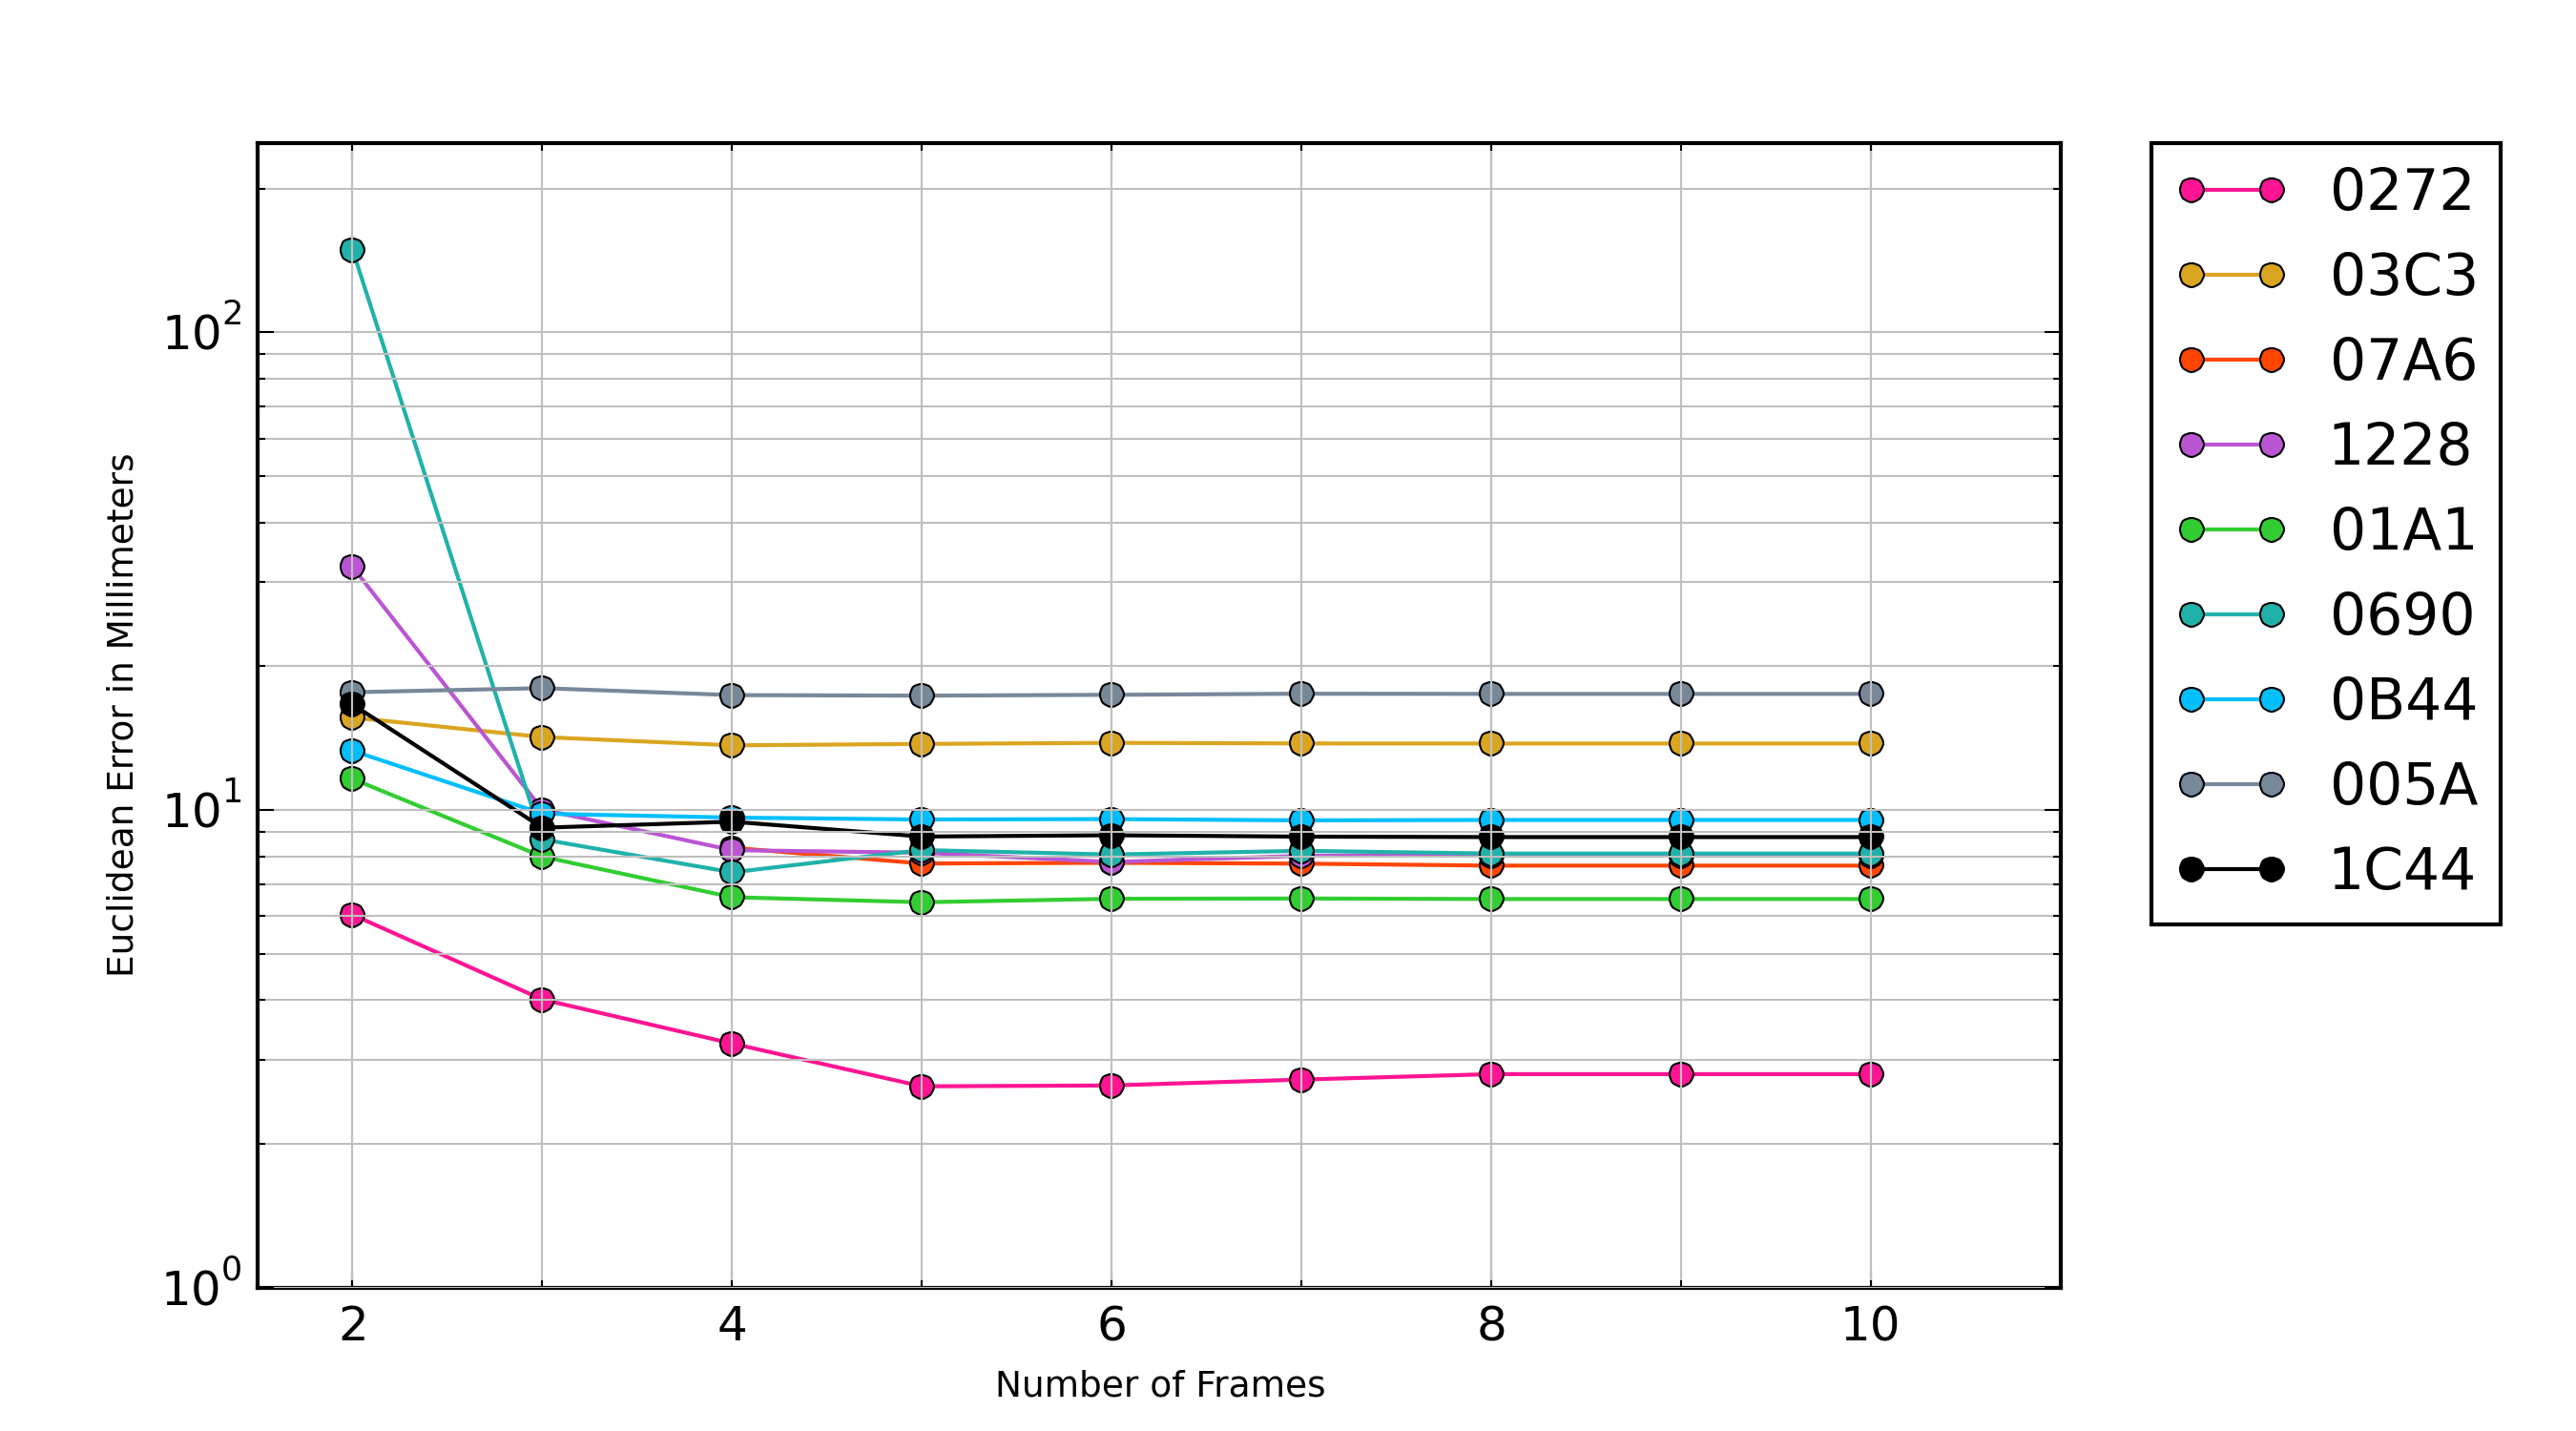
\includegraphics[width=160mm]{figures/graph_test_1}
  \caption{The euclidean distance for each marker. Each point in this figure represents the distance (euclidean error) between all four corners of that marker and ground truth corners.}\label{fig:test_1_ba}
\end{figure}

\begin{table}[H]
  \begin{tabular}{| c || c | c | c | c | c | c | c | c | c |}
      \hline
      \# BA & \nth{1} & \nth{2} & \nth{3} & \nth{4} & \nth{5} & \nth{6} & \nth{7} & \nth{8} & \nth{9} \\ \hline \hline
      Mean & 32.7776 & 10.2463 & 9.3335 & 9.1859 & 9.1667 & 9.2081 & 9.1938 & 9.1938 & 9.1938 \\ \hline
      SD & 44.4860 & 3.9315 & 3.8680 & 3.9815 & 4.0118 & 4.0023 & 3.9919 & 3.9919 & 3.9919 \\ \hline
  \end{tabular}
  \caption{The mean and standard deviation of error for all markers in each step of execution of bundle adjustment} \label{tab:test_1_ba}
\end{table}

‌‌‌‌Both \autoref{fig:test_1_ba} and \autoref{tab:test_1_ba} illustrates the tremendous impact of bundle adjustment on the raw input data. After the second bundle adjustment the mean error for all markers drops from 32.7776 milliliter to 10.2463 milliliter. Data inconsistencies also decreases from 44.4860 to 3.9315. After the second bundle adjustment, the speed of convergence get slow and it becomes stable on 9.1938 milliliters and 3.9919 milliliters for mean and standard deviation after the seventh bundle adjustment. 

\subsection{Test 2}
\begin{figure}[H]
  \centering
  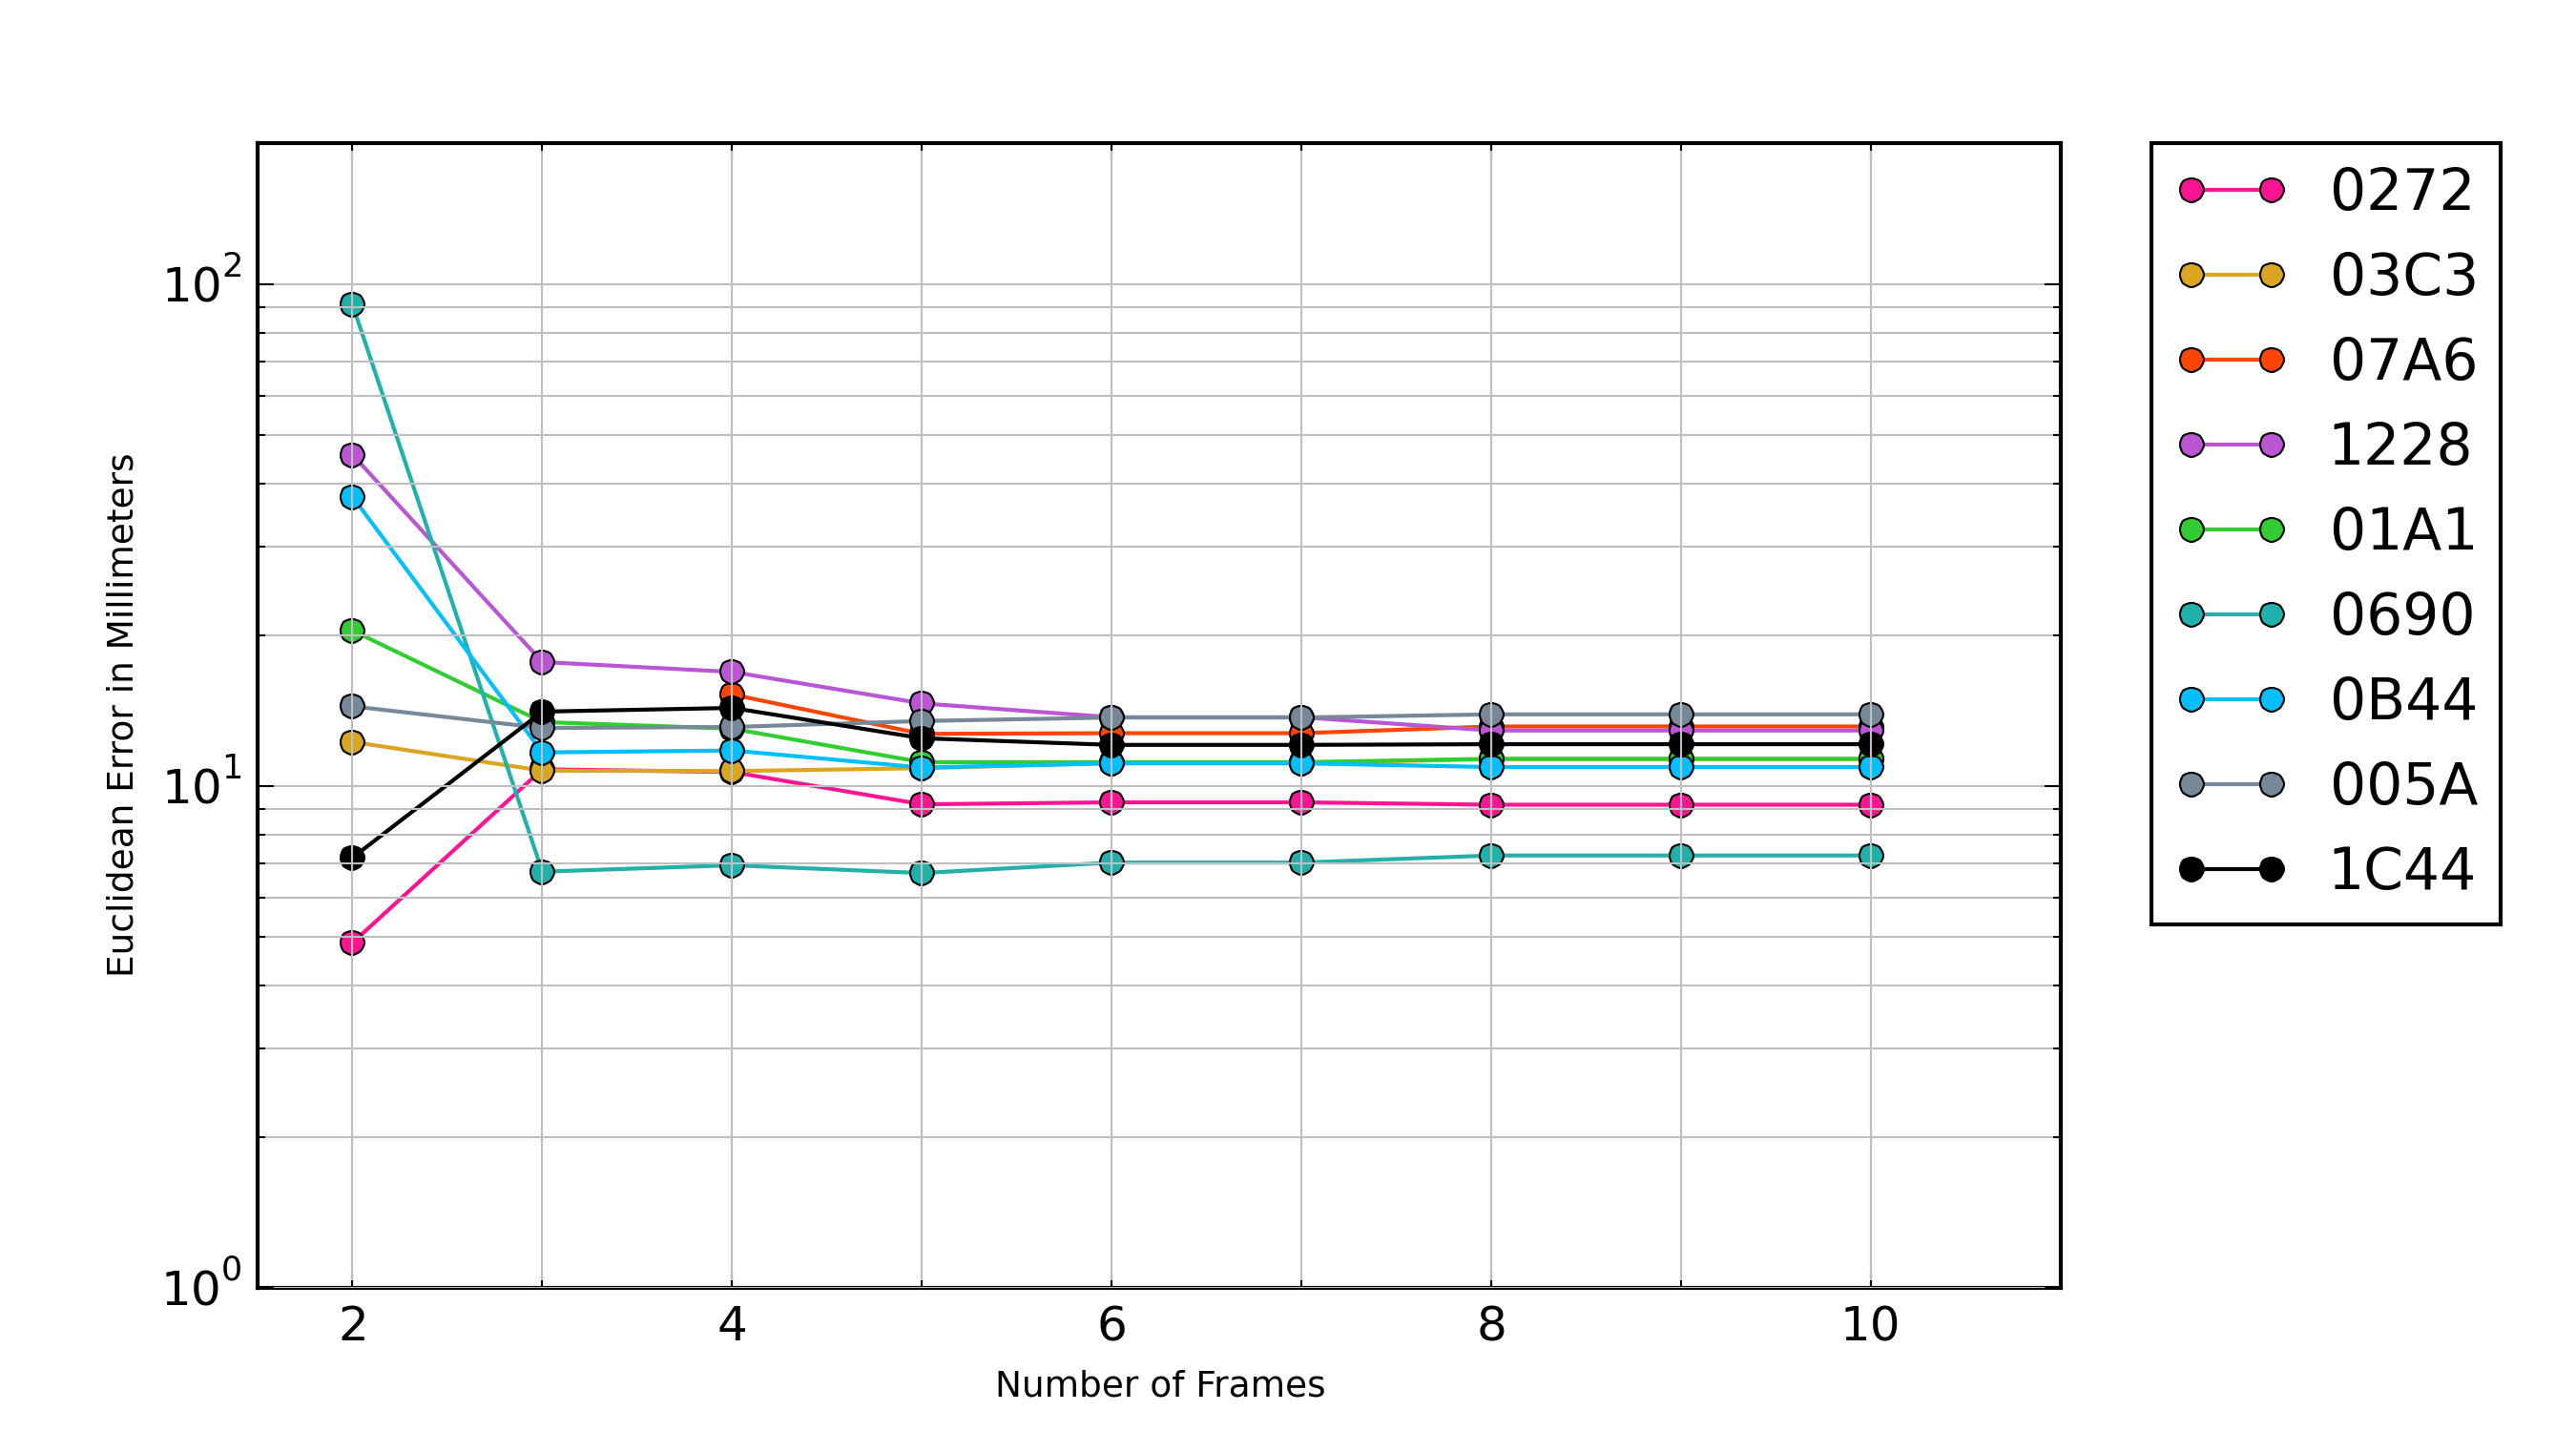
\includegraphics[width=160mm]{figures/graph_test_2}
  \caption{The euclidean distance for each marker. Each point in this figure represents the distance (euclidean error) between all four corners of that marker and ground truth corners.}\label{fig:test_2_ba}
\end{figure}

\begin{table}[H]
  \begin{tabular}{| c || c | c | c | c | c | c | c | c | c |}
      \hline
      \# BA & \nth{1} & \nth{2} & \nth{3} & \nth{4} & \nth{5} & \nth{6} & \nth{7} & \nth{8} & \nth{9} \\ \hline \hline
      Mean & 29.2014 & 12.2687 & 12.5162 & 11.3382 & 11.3243 & 11.3243 & 11.3401 & 11.3401 & 11.3401 \\ \hline
      SD & 26.9939 & 2.9500 & 2.7568 & 2.2331 & 2.0157 & 2.01567 & 1.9501 & 1.9501 & 1.9501 \\ \hline
  \end{tabular}
  \caption{The mean and standard deviation of error for all markers in each step of execution of bundle adjustment} \label{tab:test_2_ba}
\end{table}
